\documentclass{article}
\usepackage[utf8]{inputenc}
\usepackage{amsmath}
\usepackage{graphicx}

\title{Report 2: Linear Regression}
\author{Dang Vu Son Tung}
\date{05/05/2025}

\begin{document}

\maketitle

\section*{Objective}

The goal of this lab is to implement linear regression from scratch using gradient descent to find the optimal values of $w_0$ and $w_1$ for the equation:

\[
\hat{y} = w_1 \cdot x + w_0
\]

We use house price data from a CSV file and minimize the loss function:

\[
J = \frac{1}{2N} \sum_{i=1}^N (w_1 x_i + w_0 - y_i)^2
\]

\section*{Implementation}

The implementation was done in Python using the following steps:

\begin{itemize}
    \item Read data from CSV (`area`, `price`)
    \item Initialize $w_0 = 0.0$, $w_1 = 1.0$
    \item Run gradient descent to minimize the loss
    \item Print intermediate values for each step
\end{itemize}

\section*{Results}

After 50 iterations with learning rate $r = 0.0001$, the results are:

\begin{itemize}
    \item Final $w_0 \approx 0.4050$
    \item Final $w_1 \approx 15.2961$
    \item Final Loss $\approx 90.7669$
\end{itemize}

We also plotted the fitted line over the scatter plot of data.

\section*{Learning Rate Analysis}

We experimented with three learning rates: 0.001, 0.0005, 0.0001. The loss convergence is shown below:

\begin{itemize}
    \item $r = 0.001$: fast convergence, stable
    \item $r = 0.0005$: slower but stable
    \item $r = 0.0001$: slowest, but still converging correctly
\end{itemize}

\begin{center}
    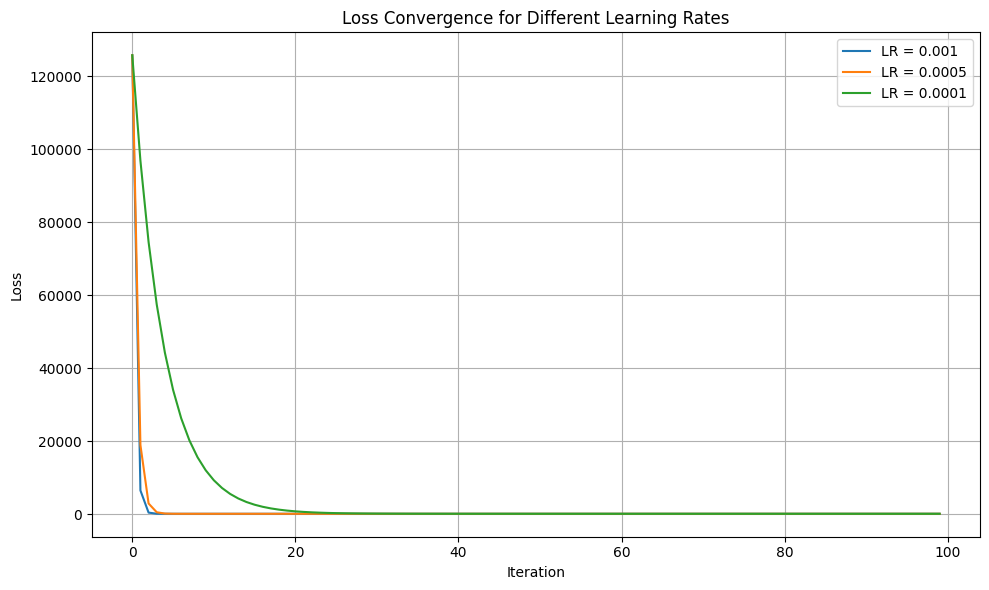
\includegraphics[width=0.7\textwidth]{loss_plot.png}
\end{center}

\section*{Conclusion}

The gradient descent method successfully optimized the weights for linear regression. The learning rate plays a crucial role in convergence speed and stability.

\end{document}
